\documentclass[./../main.tex]{subfiles}
\graphicspath{{img/}}

\begin{document}
    \color{blue}
    \begin{exercise}[Extra (valor: +2pt): Configuración electrónica de átomos multielectrónicos]
        Utilizando el Principio de Aufbau y la Regla de Madelung, construye la configuración electrónica de los siguientes átomos:

        \begin{enumerate}[threecol]
            \item Cobre (\ch{Cu}, \(Z = 29\)).
            \item Arsénico (\ch{As}, \(Z = 33\)).
            \item Neodimio (\ch{Nd}, \(Z = 60\)).
            \item Oro (\ch{Au}, \(Z = 79\)).
            \item Radón (\ch{Rn}, \(Z = 86\)).
            \item Neptunio (\ch{Np}, \(Z = 93\)).
        \end{enumerate}

        Ahora compara tus respuestas con las configuraciones electrónicas reportadas en el libro ``Physics of Atoms and Molecules''  de B.H. Bransden y C.J. Joachain (en la primera edición de este libro véase la Tabla 7.2 de la página 302).
        ¿Coinciden tus respuestas con las reportadas en el libro? En los casos en los que no coincidan explica cualitativamente porqué.

        \color{black}
        \begin{solution}
            Para construir la configuración electrónica de los diferentes átomos a partir del Principio de Aufbau y la Regla de Madelung, recordando que el Principio de Aufbau nos dice que los diferentes orbitales deben llenarse de menor a mayor energía respetando el principio de exclusión de Pauli y además nos dice que los orbitales deben llenarse por completo antes de comenzar a llenar el siguiente orbital. Por otro lado, la Regla de Madelung nos dice que la energía crece con \(n + \ell\); para dos capas con el mismo valor de \(n + \ell\), la capa con menor \(n\) se llena primero.

            Ambas reglas se pueden resumir en el siguiente diagrama:

            \begin{figure}[htb]
                \centering
                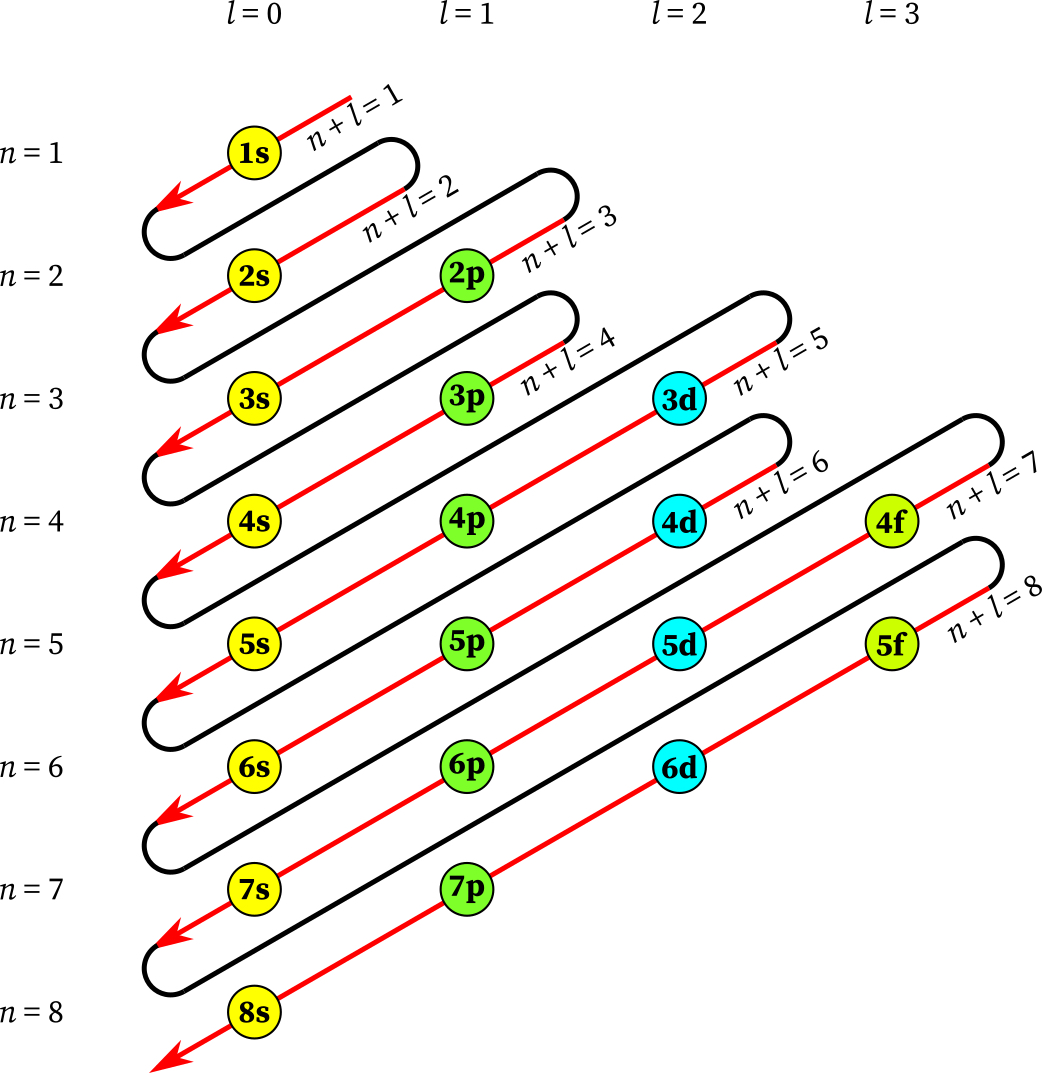
\includegraphics[scale=0.25]{1.LlenadoOrbitales}
                \caption{Diagrama de llenado de orbitales (capas).}
                \label{fig:llenado-de-orbitales}
            \end{figure}

            Además, es necesario recordar que el máximo número de electrones por orbital es de \(2(2\ell + 1)\), tal que

            \begin{align*}
                \ell &= 0 \,(\text{orbital s})\, \text{el número máximo de electrones es}\, 2,\\
                \ell &= 1 \,(\text{orbital p})\, \text{el número máximo de electrones es}\, 6,\\
                \ell &= 2 \,(\text{orbital d})\, \text{el número máximo de electrones es}\, 10,\\
                \ell &= 3 \,(\text{orbital f})\, \text{el número máximo de electrones es}\, 14.
            \end{align*}

            Por lo que, las configuraciones electrónicas de los diferentes átomos son:

            \begin{enumerate}
                \item Cobre (\ch{Cu}, \(Z = 29\))
                
                \begin{equation*}
                    \writeelconf{2,2+6,2+6+9,2},
                \end{equation*}

                o bien,

                \begin{equation*}
                    \ch{[Ar]}\writeelconf{,,++9,2}.
                \end{equation*}

                Comparando con aquella reportando en el libro,

                \begin{equation*}
                    \ch{[Ar]}\writeelconf{,,++10,1},
                \end{equation*}

                \idest las configuraciones no coinciden. De la \cref{fig:first-excites-states-helium} sabemos que el orbital \(3d\) tiene menor energía que el orbital \(4s\), lo cual nos indica que es más susceptible a ser llenado primero.

                \item Arsénico (\ch{As}, \(Z = 33\))
                
                La configuración electrónica de este átomo es

                \begin{equation*}
                    \ch{[Ar]}\writeelconf{,,++10,2+3}.
                \end{equation*}

                Y comparándola con la del libro podemos confirmar que se llega a la misma configuración.

                \item Neodimio (\ch{Nd}, \(Z = 60\))
                
                La configuración electrónica de este átomo es

                \begin{equation*}
                    \ch{[Ar]}\writeelconf{,,++10,2+6+10+4,2+6,2},
                \end{equation*}

                o bien,

                \begin{equation*}
                    \ch{[Xe]}\writeelconf{,,,+++4,,2}.
                \end{equation*}

                Y notamos que esta configuración es la misma que la reportada en el libro.

                \item Oro (\ch{Au}, \(Z = 79\))
                
                La configuración electrónica para el \ch{Au} es

                \begin{equation*}
                    \ch{[Xe]}\writeelconf{,,,+++14,++9,2}.
                \end{equation*}

                Y la reportada en el libro es

                \begin{equation*}
                    \ch{[Xe]}\writeelconf{,,,+++14,++10,1}.
                \end{equation*}

                Fijándonos nuevamente en la \cref{fig:first-excites-states-helium}, notamos que el orbital que tiene mayor energía el 6s y el orbital con menor energía el 5d, por lo que es más probable que este se llene primero.
                
                \item Radón (\ch{Rn}, \(Z = 86\))
                
                La configuración electrónica para el \ch{Rn} es

                \begin{equation*}
                    \ch{[Xe]}\writeelconf{,,,+++14,++10,2+6}.
                \end{equation*}

                Comparándola con la del libro, notamos que es la misma.
                
                \item Neptunio (\ch{Np}, \(Z = 93\))
                
                La configuración electrónica para el \ch{Np} es

                \begin{equation*}
                    \ch{[Xe]}\writeelconf{,,,+++14,++10+5,2+6,2},
                \end{equation*}

                o bien,

                \begin{equation*}
                    \ch{[Rn]}\writeelconf{,,,,+++5,,2}.
                \end{equation*}

                Mientras que la reportada en el libro es

                \begin{equation*}
                    \ch{[Rn]}\writeelconf{,,,,+++4,++1,2}.
                \end{equation*}

                Análogamente al caso del \ch{Au} notamos que el orbital con menor energía es el 5f; sin embargo, eso implicaría una transición prohibida, por lo que es más susceptible que el orbital cuya energía es mayor que la del 5f, pero menor que la del 7s, se llene primero, \idest el 6d.
            \end{enumerate}        
        \end{solution}
    \end{exercise}
\end{document}